\documentclass[a4paper, 10pt]{article}
\usepackage{amsmath}
\usepackage{amssymb}
\usepackage[justification=raggedright,singlelinecheck=false]{caption}
\usepackage{graphicx}
\usepackage{float}
\usepackage[margin=0.5in]{geometry}
\usepackage{hyperref}
\usepackage{subcaption}
\usepackage{tabularx}

\title{Gaussian Processes for Time Series}
\date{\today}
\author{Raphaela Azar and Sbonelo Gumede}

\begin{document}

   \maketitle

   \section*{Introduction}

      \begin{table}[H]
         \raggedright
         \renewcommand{\arraystretch}{1.3}
         \begin{tabularx}{\textwidth}{|l|l|X|l|}
         \hline
         \text{Variable} & \text{Feature Name} & \text{Feature Description} & \text{Unit} \\
         \hline
         \(\text{NO}_{2}\) & Nitrogen dioxide & A harmful gas from vehicles and industry. & \(\mu\text{g}/\text{m}^{3}\) \\
         \hline
         \(\text{PM}_{10}\) & Particulate matter 10 & Small inhalable dust particles. & \(\mu\text{g}/\text{m}^{3}\) \\
         \hline
         \(\text{SO}_{2}\) & Sulphur dioxide & Mainly from burning fossil fuels. & \(\mu\text{g}/\text{m}^{3}\) \\
         \hline
         Direction & Wind direction & Indicates where the wind is coming from. & Degrees (0–360°) \\
         \hline
         Speed & Wind speed & How fast the wind is moving. & m/s \\
         \hline
         \end{tabularx}
         \caption{Description of variables used in the analysis.}
      \end{table}

      \subsection*{Exploratory Data Analysis}
         \begin{figure}[H]
            \raggedright
            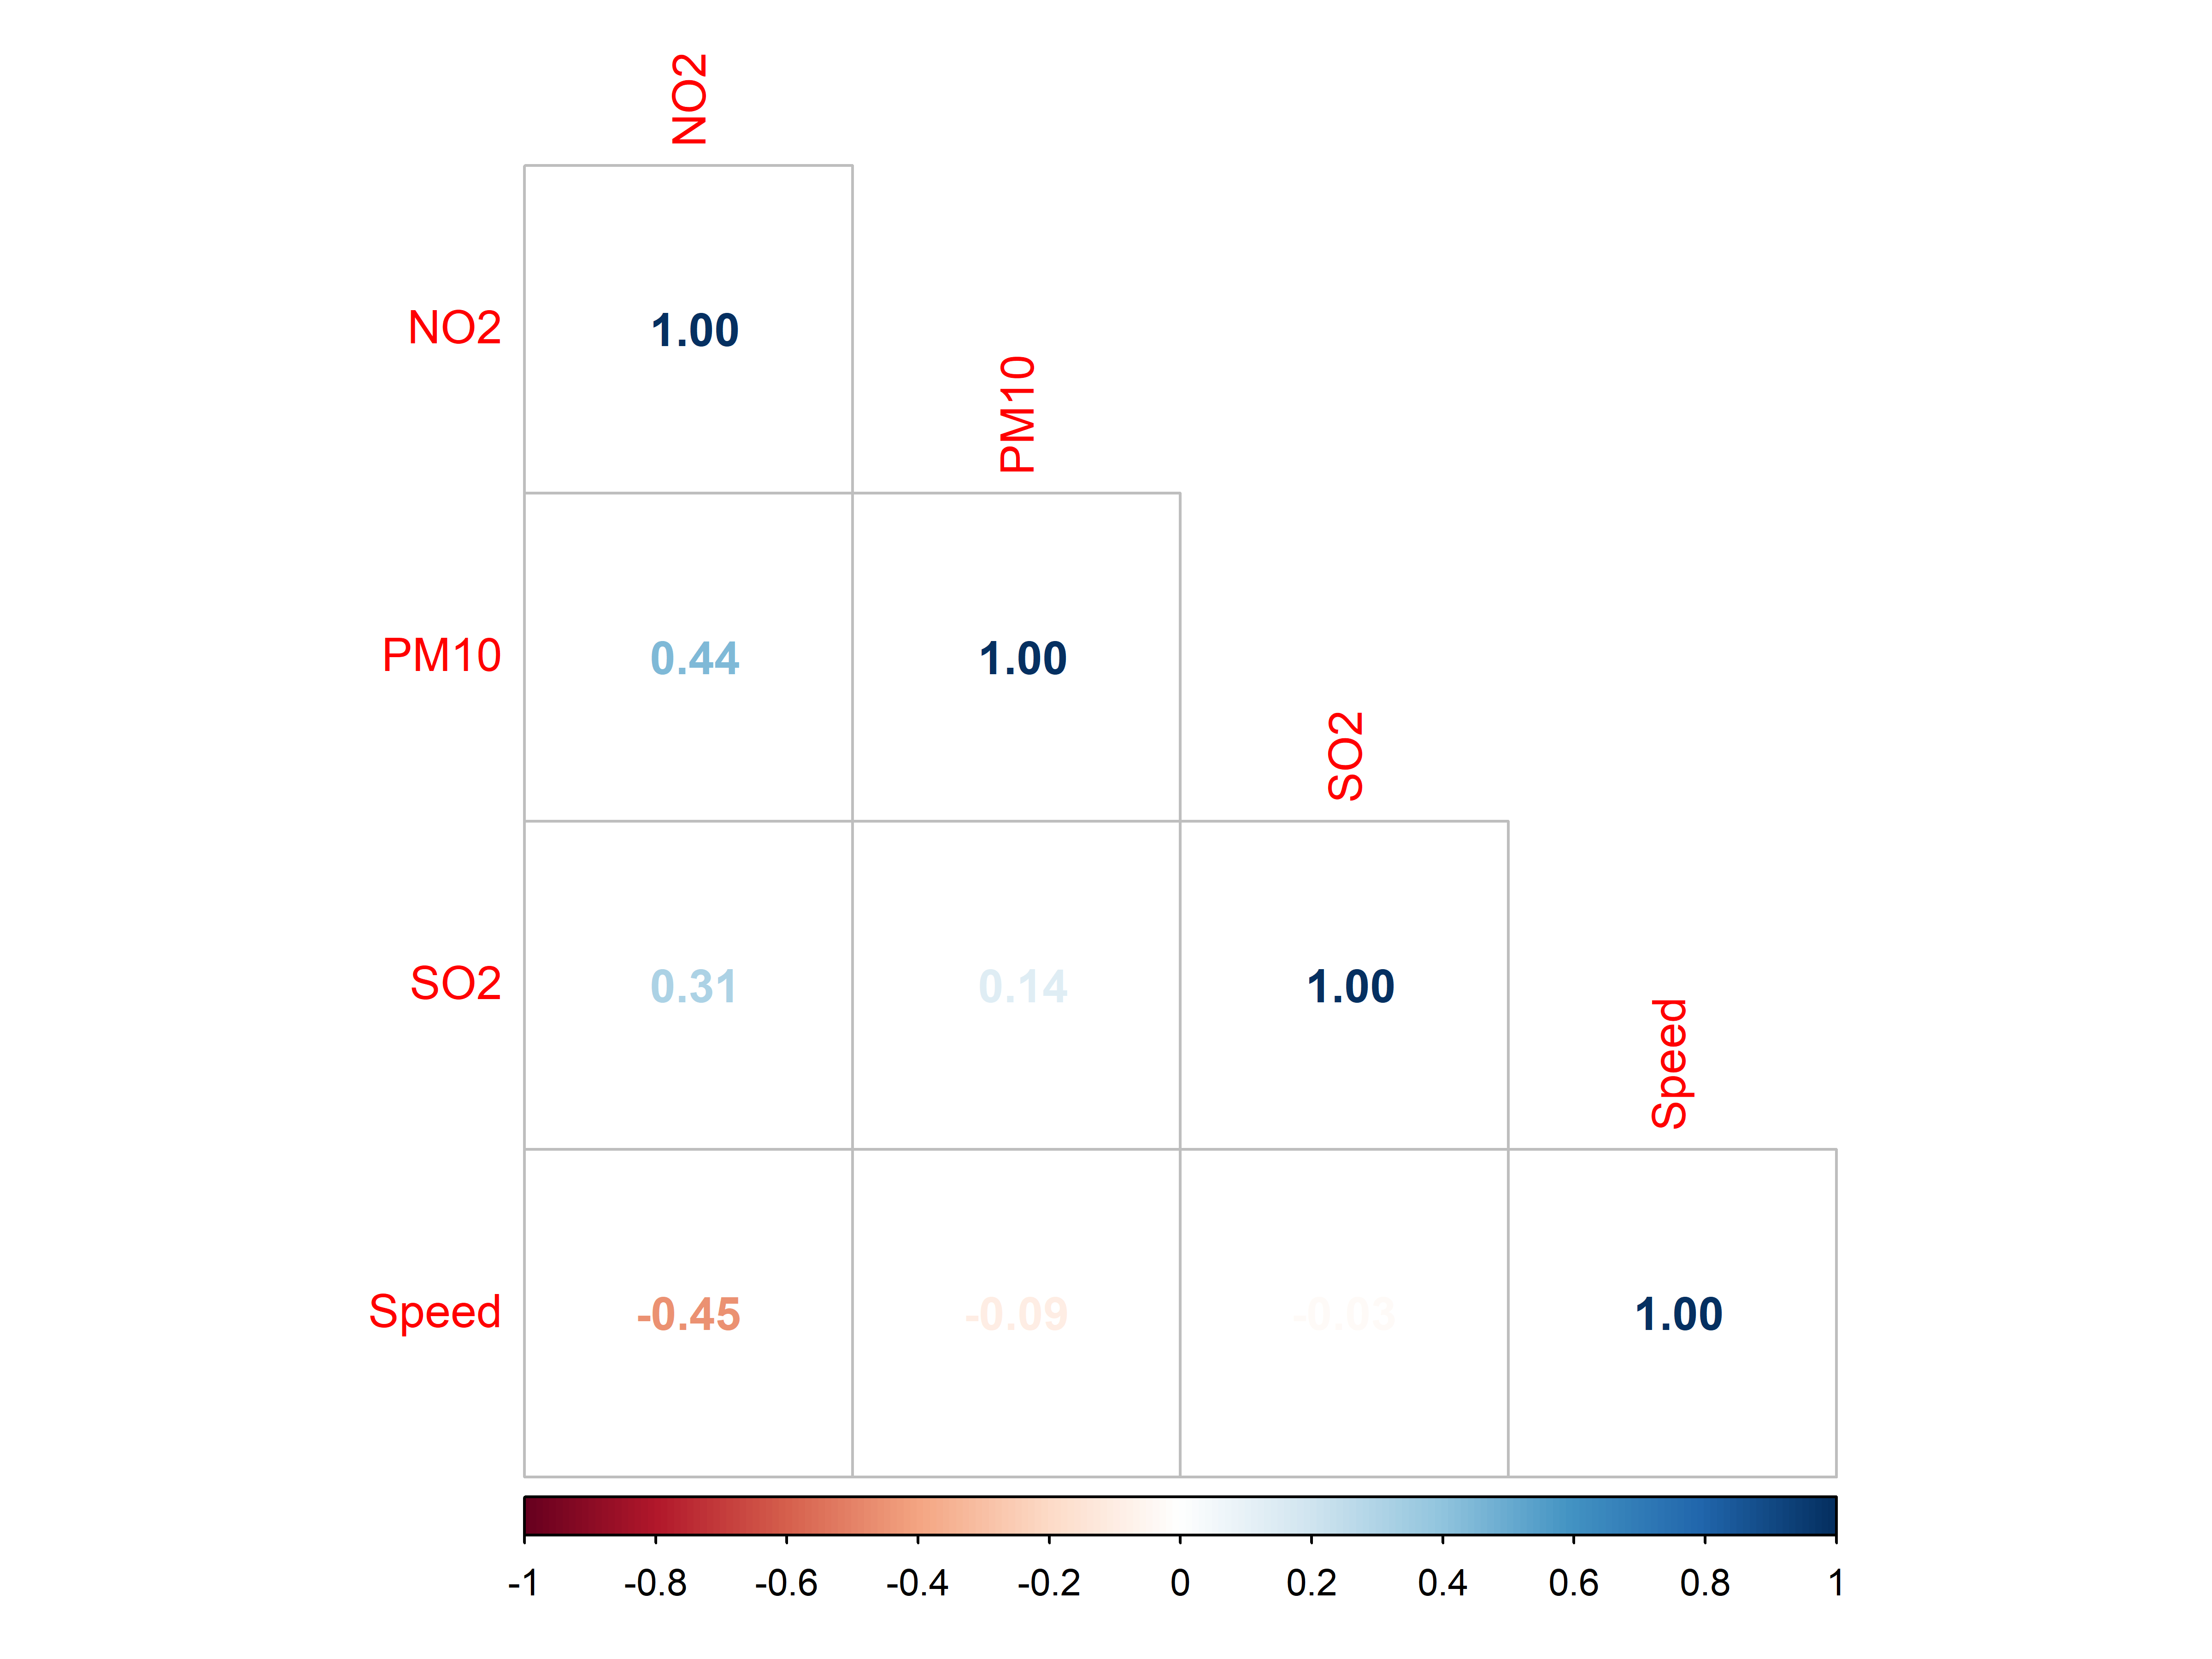
\includegraphics[width=0.48\linewidth]{../images/corrplot_2019.png}
            \caption{Correlation plot of the variables.}
         \end{figure}

         \begin{figure}[H]
            \centering
            \begin{subfigure}[t]{0.48\linewidth}
               \centering
               \includegraphics[width=\linewidth]{../images/PM10_hist_2019.png}
               \caption{Histogram of $\text{PM}_{10}$.}
            \end{subfigure}
            \hfill
            \begin{subfigure}[t]{0.48\linewidth}
               \centering
               \includegraphics[width=\linewidth]{../images/SO2_hist_2019.png}
               \caption{Histogram of $\text{SO}_{2}$.}
            \end{subfigure}
            \vfill
            \begin{subfigure}[t]{0.48\linewidth}
               \centering
               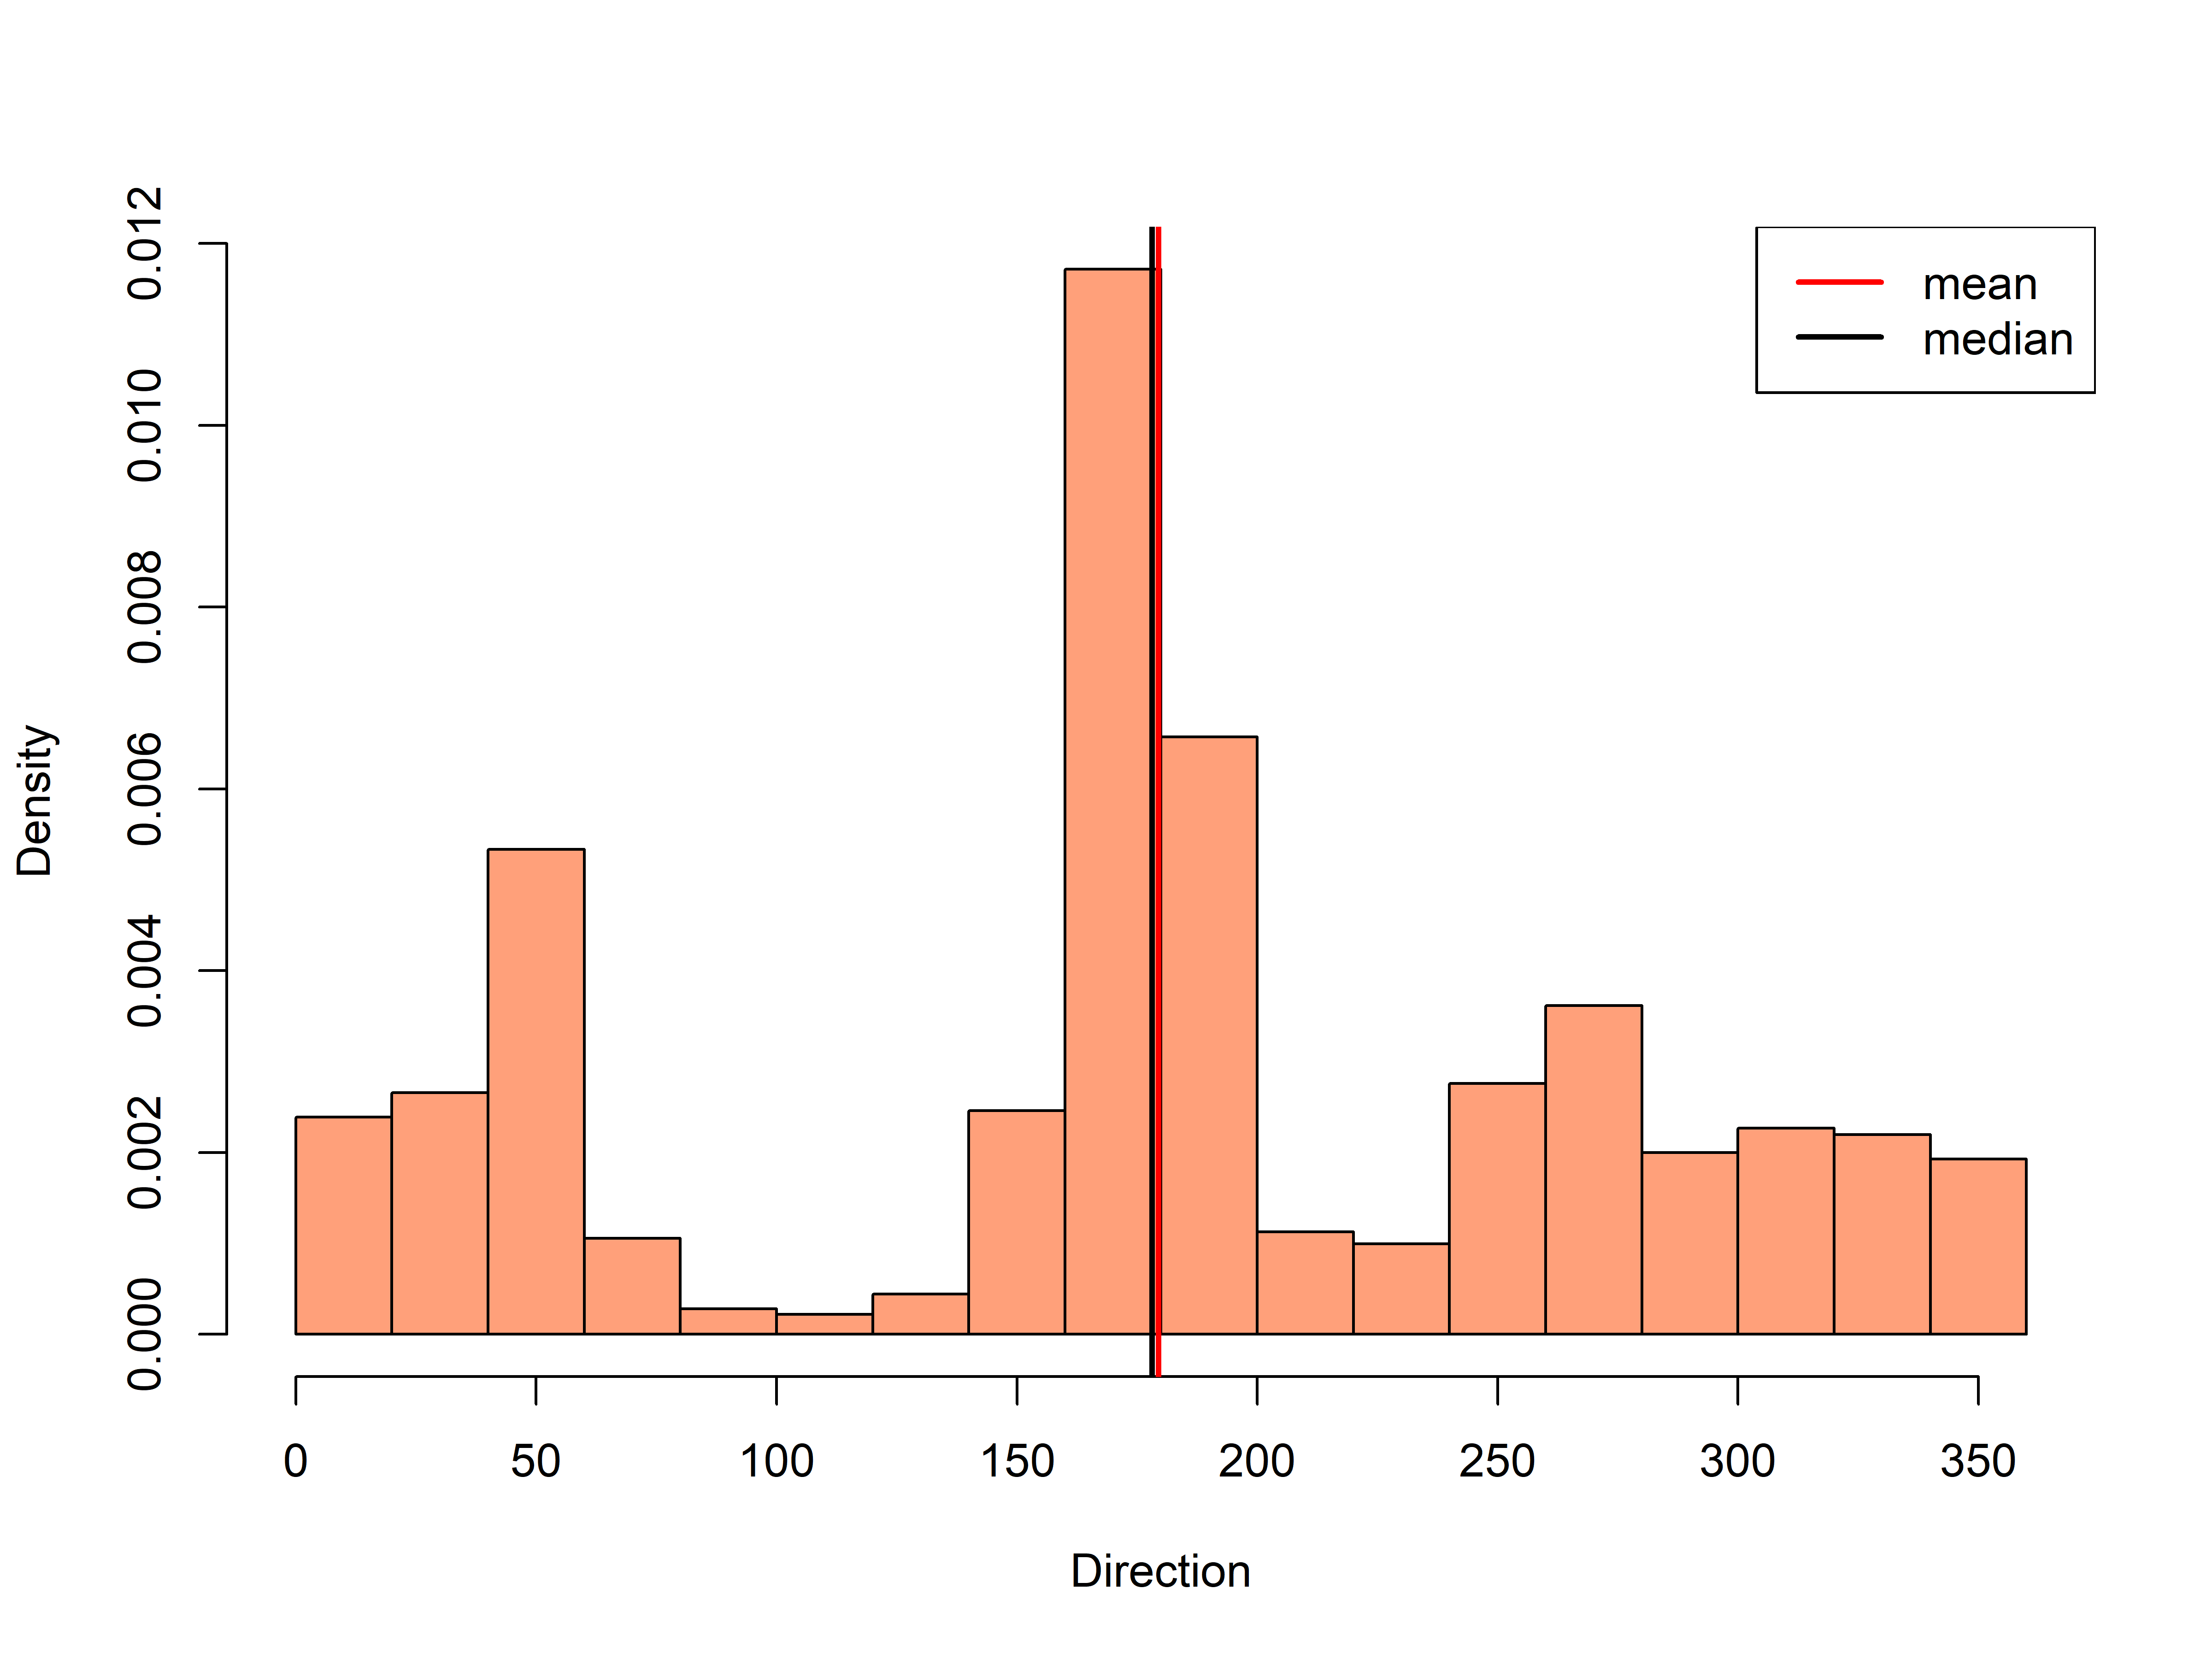
\includegraphics[width=\linewidth]{../images/direction_hist_2019.png}
               \caption{Histogram of Direction.}
            \end{subfigure}
            \hfill
            \begin{subfigure}[t]{0.48\linewidth}
               \centering
               
\includegraphics[width=\linewidth]{../images/speed_hist_2019.png}
               \caption{Histogram of Speed.}
            \end{subfigure}
         \end{figure}
         
         \begin{figure}[H]
            \centering
            \begin{subfigure}[t]{0.48\linewidth}
               \centering
               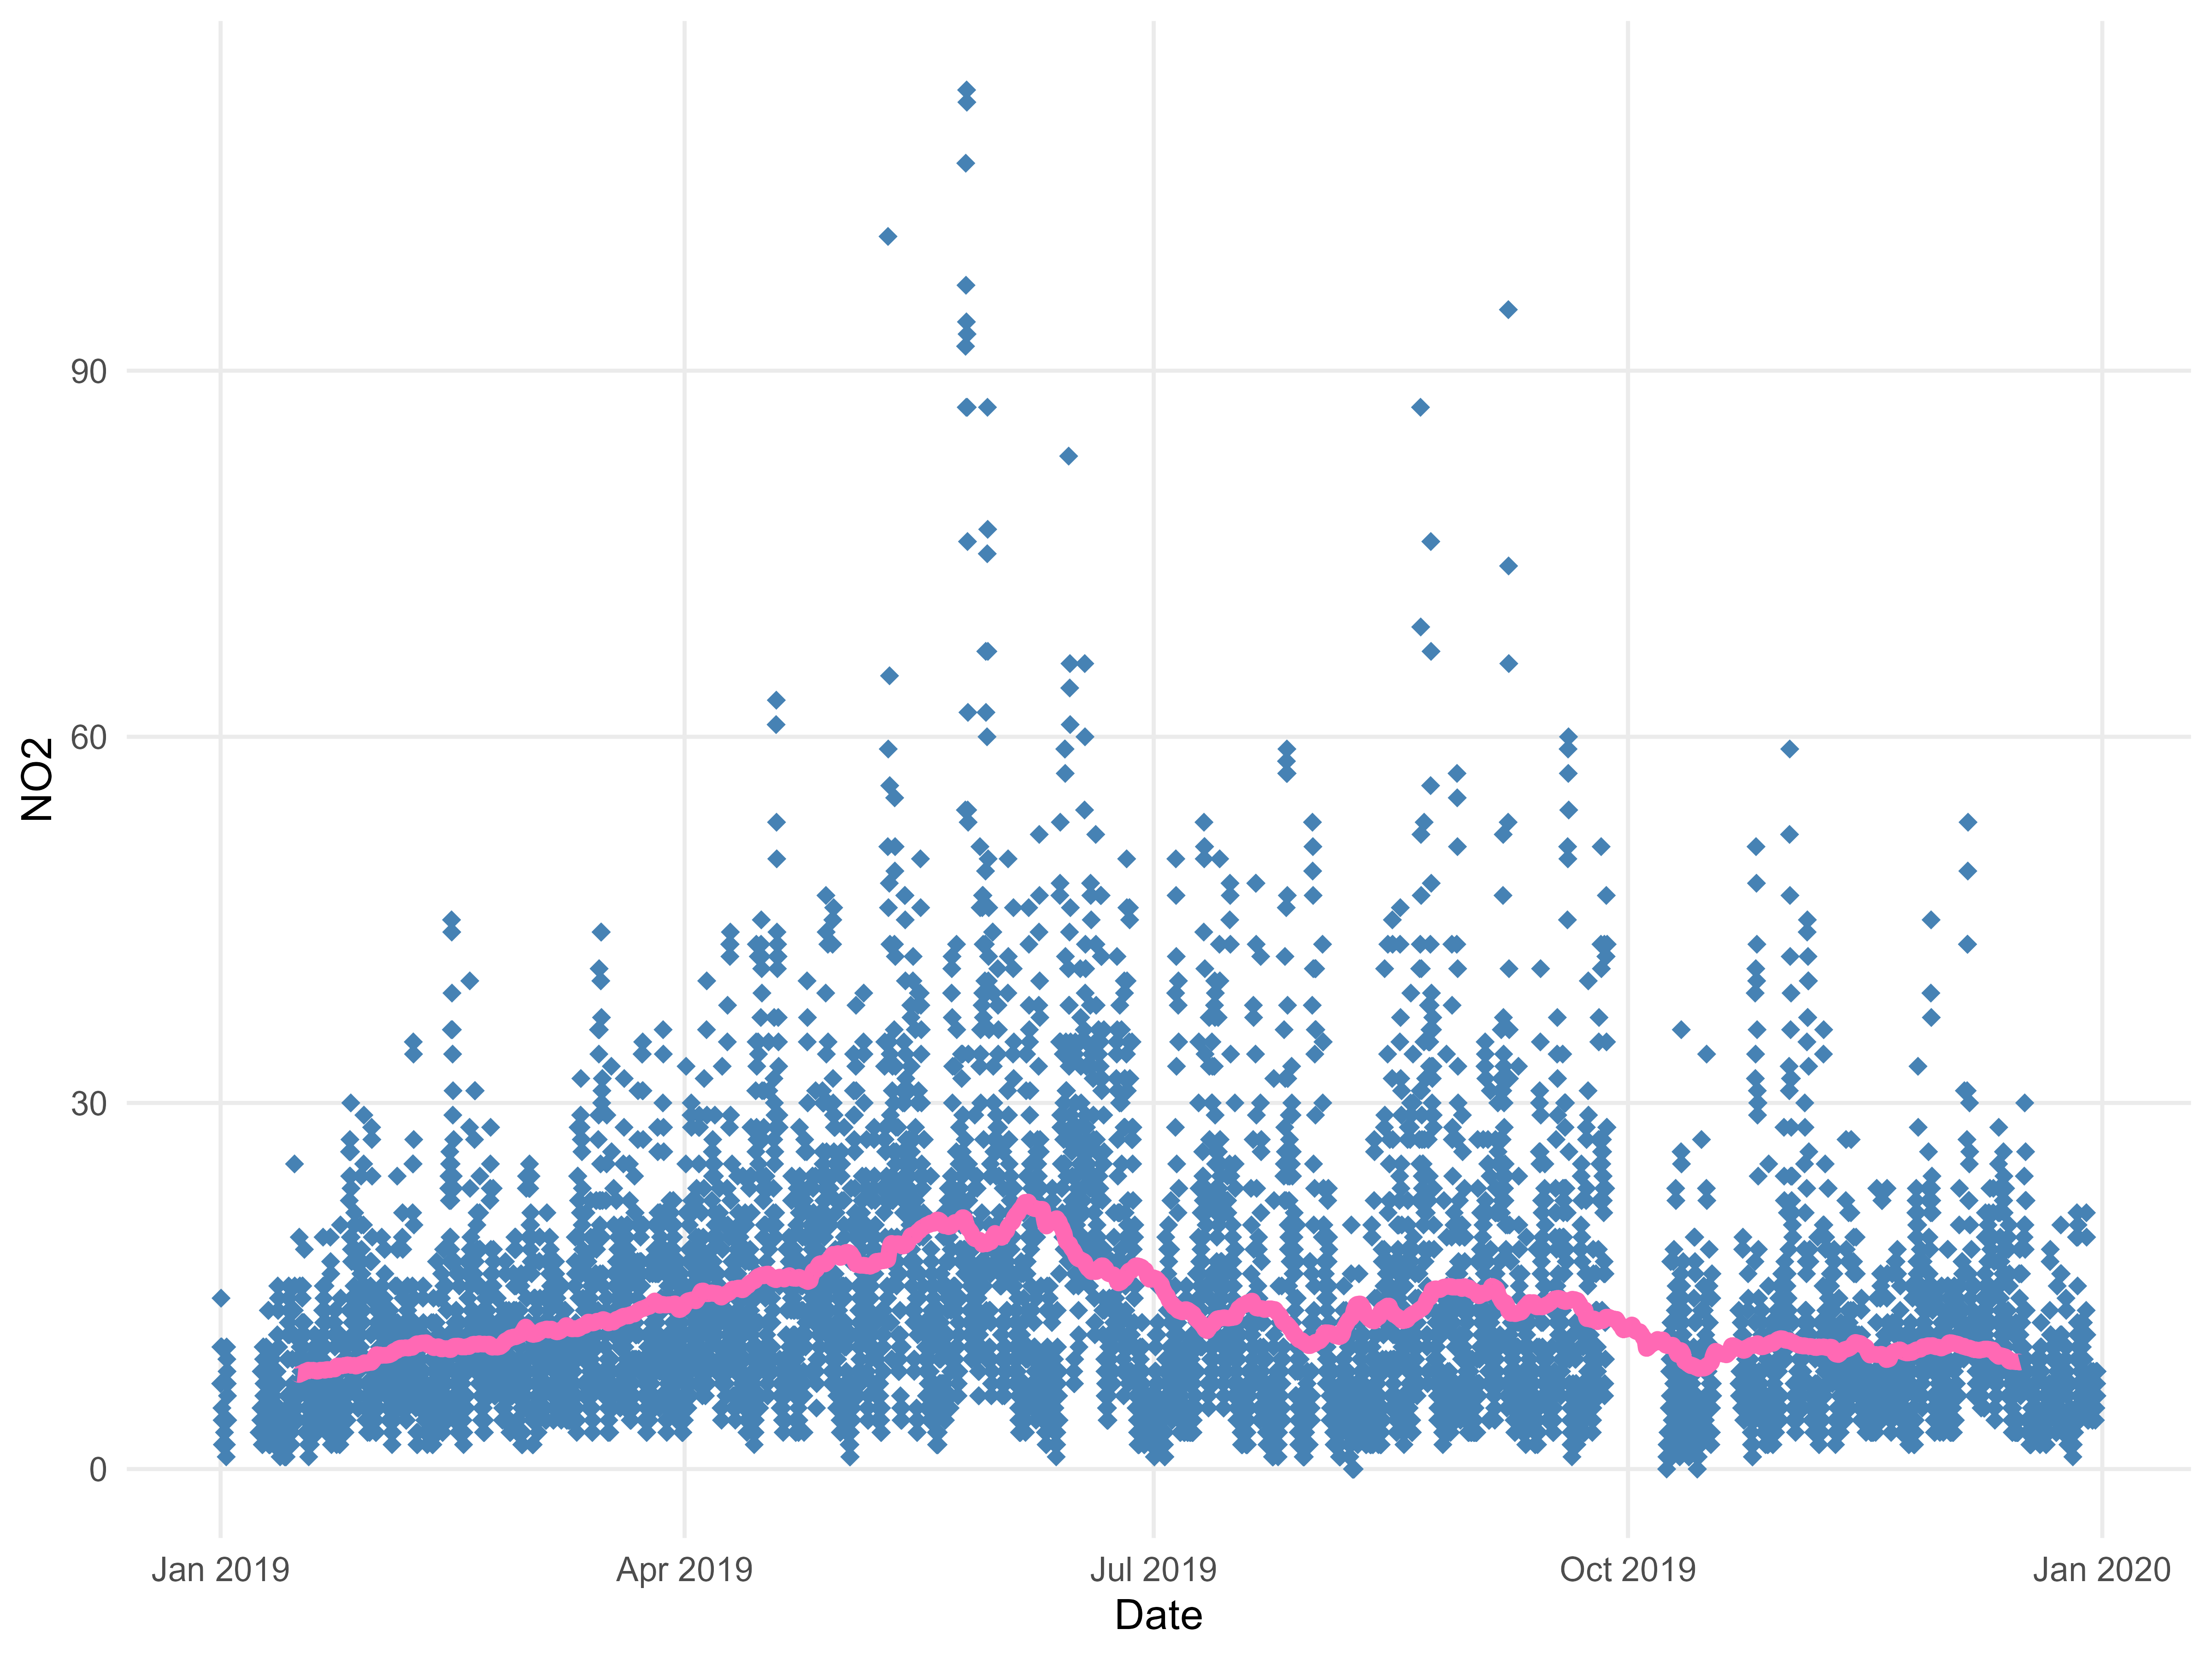
\includegraphics[width=\linewidth]{../images/no2_scatter_2019.png}
               \caption{Scatter plot of $\text{NO}_{2}$.}
            \end{subfigure}
            \hfill
            \begin{subfigure}[t]{0.48\linewidth}
               \centering
               
\includegraphics[width=\linewidth]{../images/no2_hist_2019.png}
               \caption{Histogram of $\text{NO}_{2}$.}
            \end{subfigure}
         \end{figure}

         \begin{figure}[H]
            \centering
            \begin{subfigure}[t]{0.48\linewidth}
               \centering
               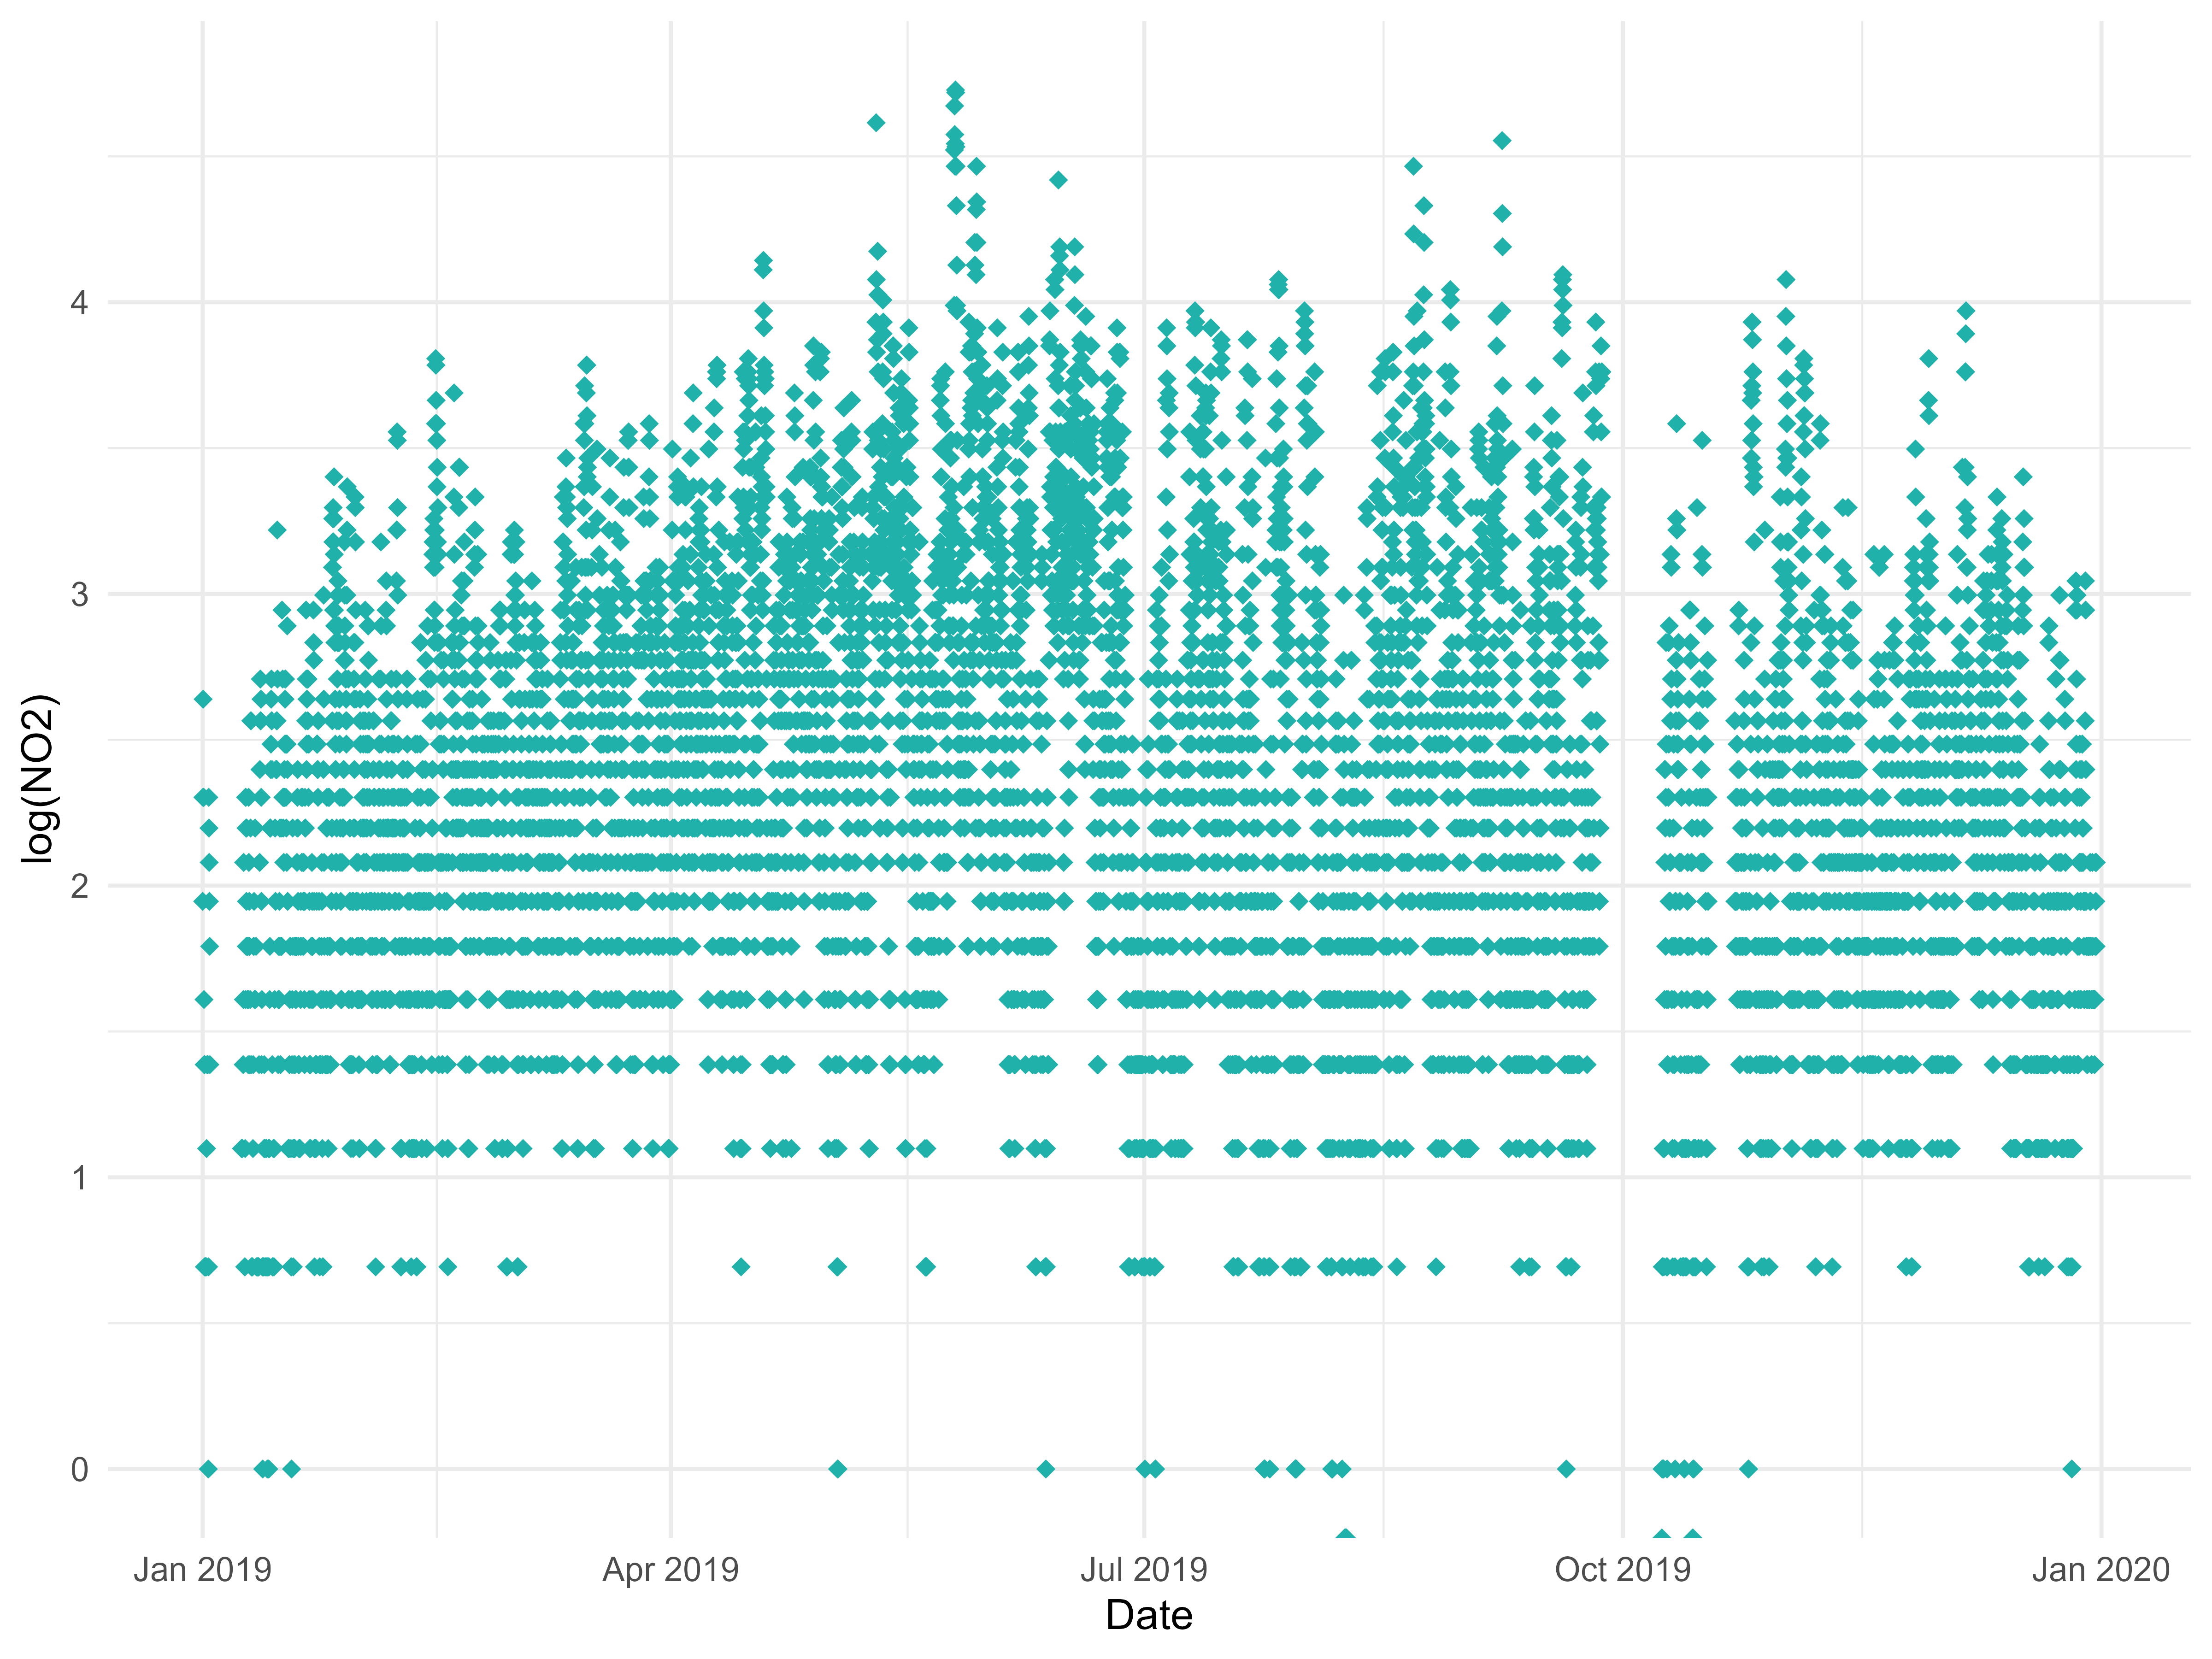
\includegraphics[width=\linewidth]{../images/log_no2_scatter_2019.png}
               \caption{Scatter plot of $log(\text{NO}_{2})$.}
            \end{subfigure}
            \hfill
            \begin{subfigure}[t]{0.48\linewidth}
               \centering
               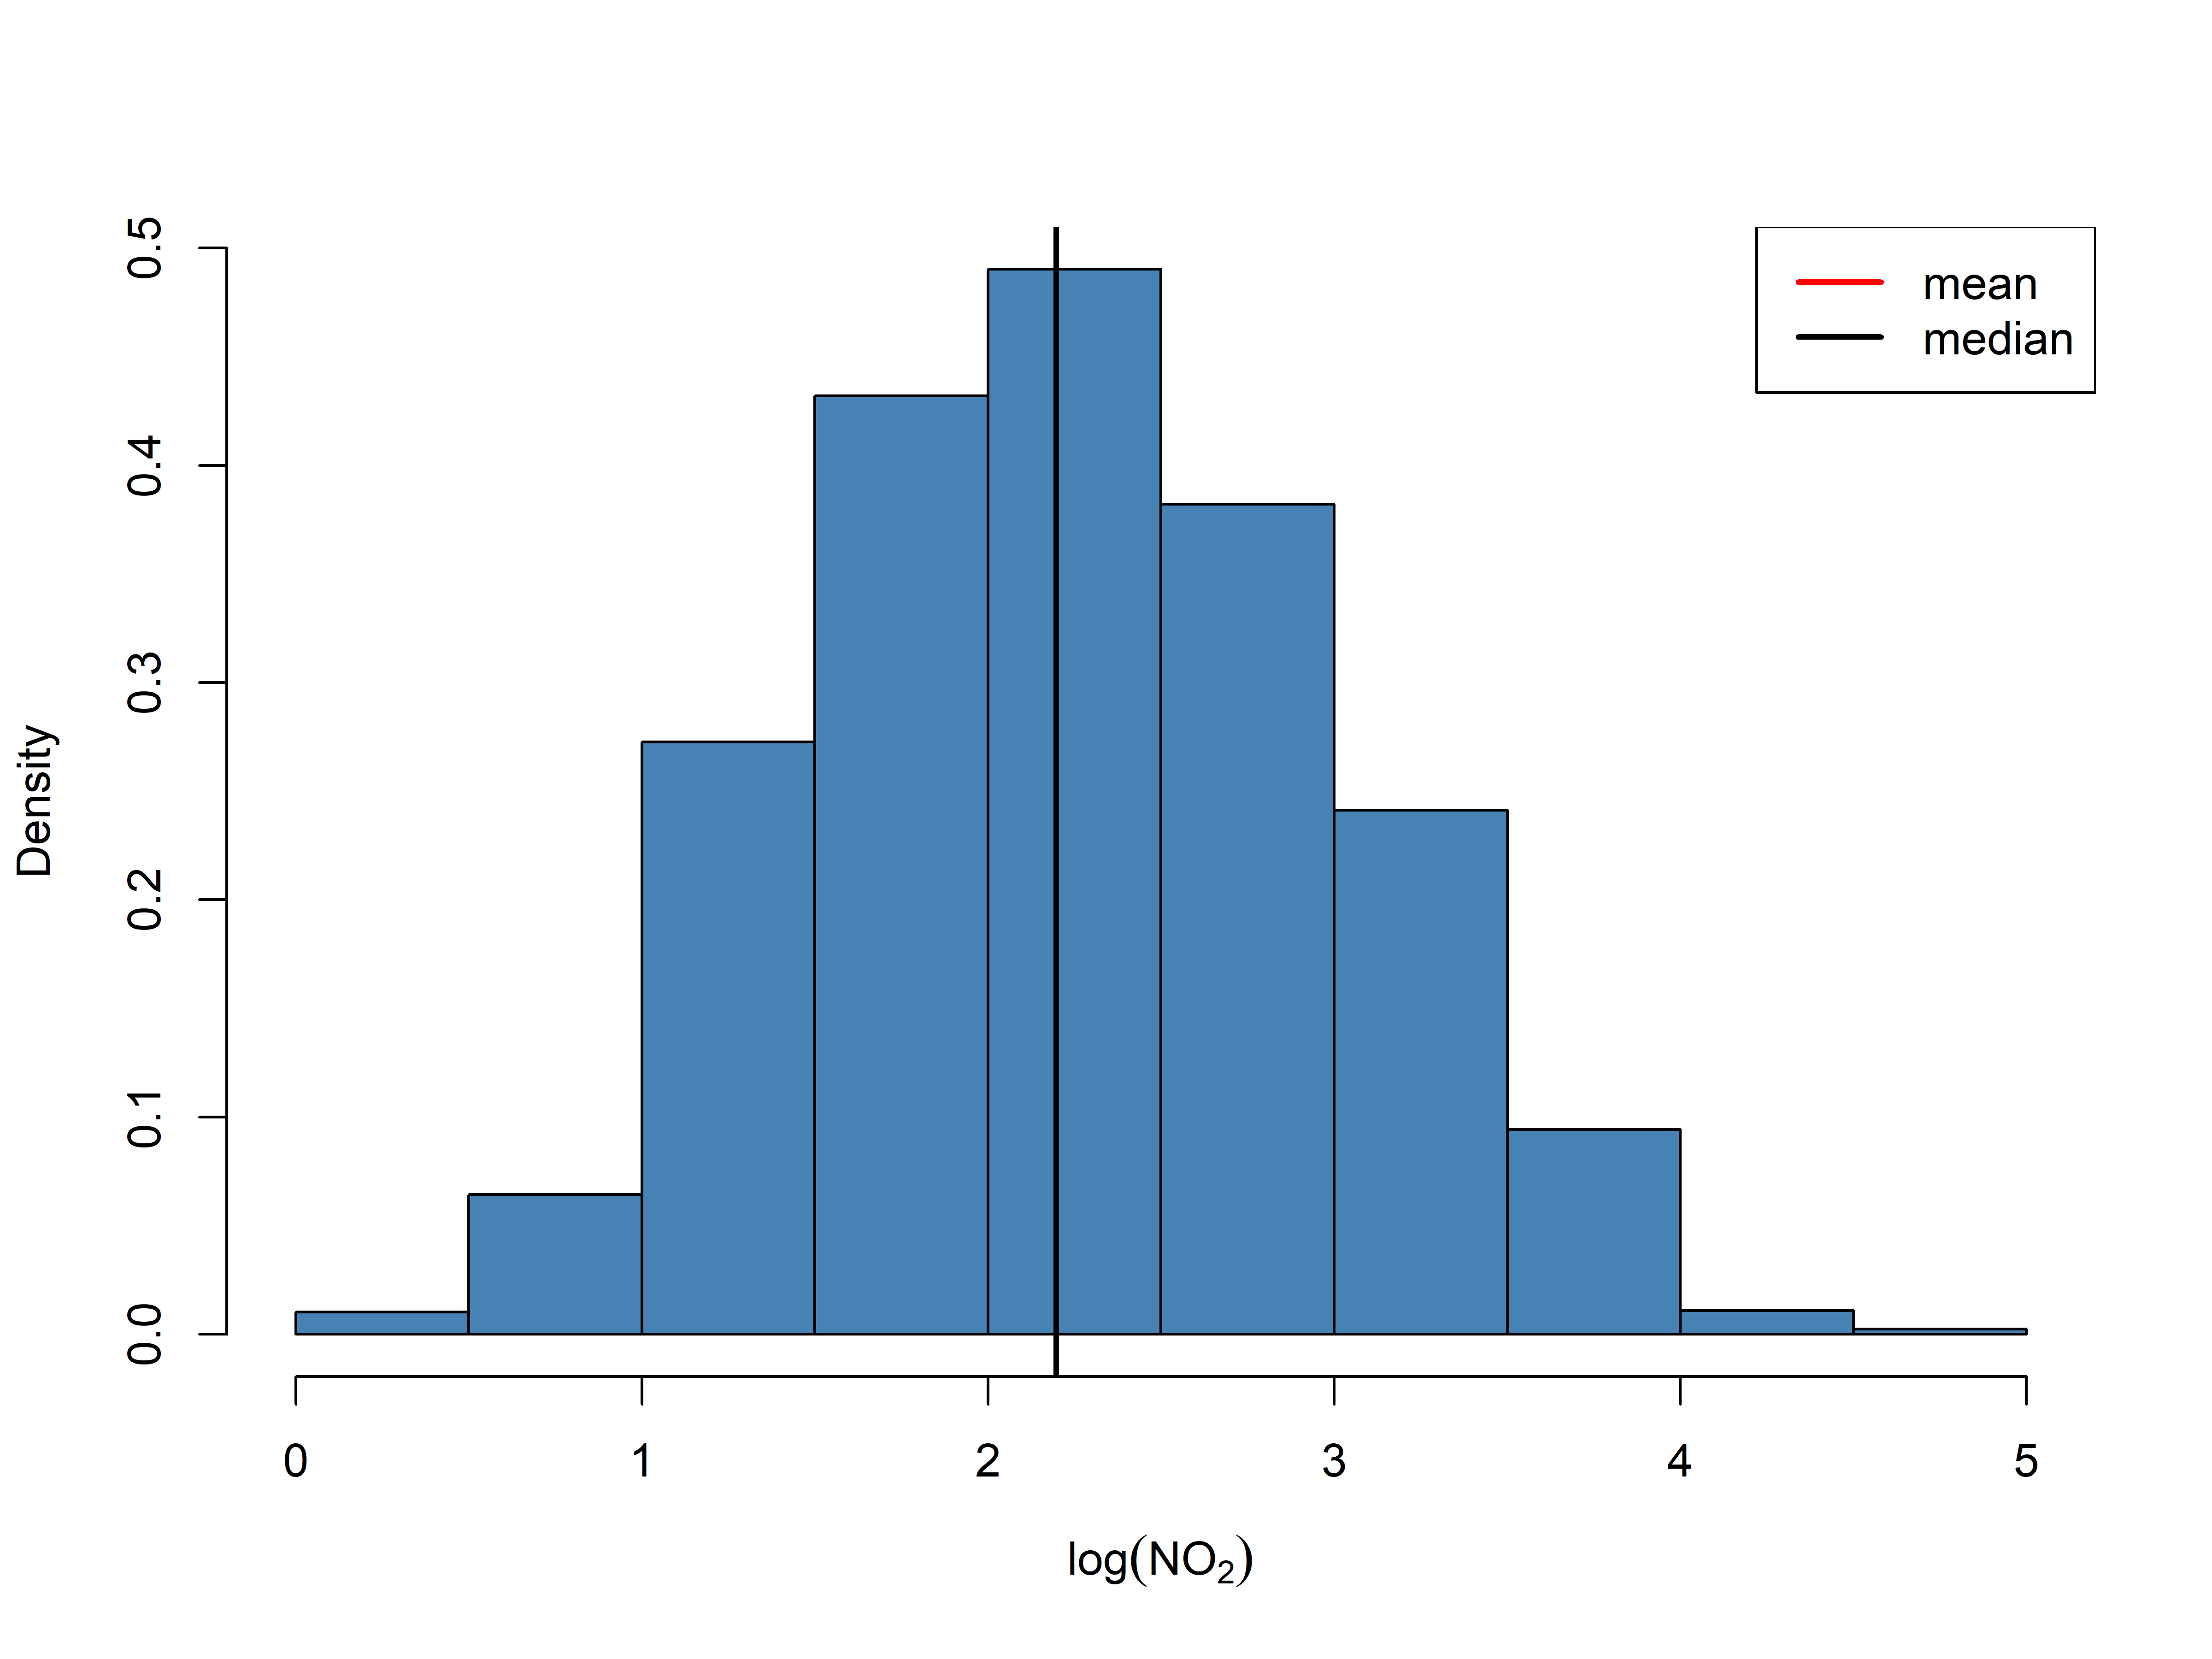
\includegraphics[width=\linewidth]{../images/log_no2_hist_2019.png}
               \caption{Histogram of $log(\text{NO}_{2})$.}
            \end{subfigure}
         \end{figure}

         Let $Y := \text{NO}_{2}$ levels in the atmosphere. 
         Notice that $Y \not\sim \mathcal{N}(\mu, \, \sigma)$ but $log(Y) \dot{\sim} \mathcal{N}(\mu, \, \sigma)$.\\
         Our Gaussian process is of the form $h(x) \sim \mathcal{N}(f(x), \, g(x)), \, x \in \mathbb{R}$.
         The resultant covariance matrix of $g(x)$ must be positive semi-definite. 
         Thus $g(x)$ must be chosen appropriately.
         The proposed model for the mean function is $f(x) = \alpha + x^{T} \beta$.
   
   \section*{References}
      \begin{enumerate}
         \item https://www.lung.org/clean-air/outdoors/what-makes-air-unhealthy/nitrogen-dioxide
      \end{enumerate}
\end{document}